\documentclass[handout]{beamer}
\mode<presentation>
\usepackage{beamerthemesplit}
\usepackage{amsmath}
\usepackage{amsthm}
\usepackage{amsfonts}
\usepackage[english]{babel}
\usepackage{amssymb}
\usepackage{etex}
\usepackage{xy}
\input xy
\xyoption{all}

%\uselanguage{spanish}
%\languagepath{spanish}


%\uselanguage{Spanish}
%\languagepath{Spanish}

\theoremstyle{plain}
\newtheorem{prop}{Proposici\'on}[section]
\newtheorem{teor}{Teorema}[section]
\newtheorem{defi}{Definici\'on}[section]
\newcommand{\coker}{\operatorname{coker}}
\renewcommand{\P}{\mathbb{P}}
\newcommand{\G}{\mathcal{G}}

\title{Rigidity, Mapping  Class Groups  and Stochastic Topology. }
\author{No\'e B\'arcenas.\\ Joint work with O. Arizmendi \\  and R.Ch\'avez C\'aliz.}
\institute{Centro de  Ciencias Matem\'aticas. \\ UNAM. }
\date{V Escuela  de  An\'alisis Topol\'ogico  de  Datos.}
\begin{document}
\begin{frame}
\titlepage
\end{frame}



\section{Rigidity}

\begin{frame}
\frametitle{What  is  rigidity?}

Surfaces. \\

We  will  associate a  group  to  a  a  surface, $Mod(S)$,  the  mapping  class  group. \pause
Rigidity: Group  homomorphisms 
$$ Mod(S) \to Mod  (S^{'})$$
are  induced  by  manipulation  of  the  given surfaces. 
\end{frame}

%The  first  one  is  an example of  non-rigidity. \\
%The  second one  is  an  example  of  a  rigid  behaviour. \pause 
%In  both  cases, the  Mapping  class  group  is  protagonist of   the  phenomena.


\begin{frame}\frametitle{Mapping  class group ?}

Let  $S$  be  a 2- dimensional  smooth  manifold without  boundary. \pause
$S$  can  be  furnished  with  a Riemannian  Metric, even with  a  complex structure. \pause Is  it  unique? \pause
NO. \pause 

\begin{figure}[h!]
	\centering
	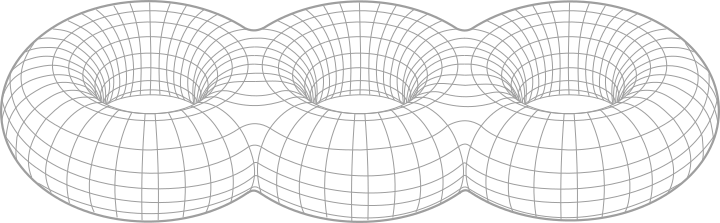
\includegraphics[scale=0.35]{CHARLA_STOCHASTIC_TOPOLOGY_MCG_CIMATNOVEMBER_2018/multitorus.png}
	\caption{Surface of gender 3}
\end{figure}

There  is  a  whole  space $T(S)$ of  complex  structures  on  $S$. \pause (Homeomorphic  to  an  euclidean Ball  of  dimension $6g-6$  if  the  surface  has  genus  $g$). \pause 

\end{frame}
\begin{frame}\frametitle{Example  of  a  non-rigid phenomenon. Continuation.}

Homeomorphisms  of  the  surface  act  on  this space: 
$$ S\overset{\varphi }{\to } S^{'}, $$ \pause 


But homeomorphisms  that  are homotopic   to the  identity fix  the  complex structure we  started with. \pause 
(These, the   ones non-homotopic  to $id$  are  responsible  for  this  non-rigid  aspect of  the  theory  of  surfaces: the  complex  structure  is  not  unique, and  there  is  a  whole  Moduli). 

\end{frame}



\begin{frame}\frametitle{Mapping Class group! }

Consider a  closed  surface. A  curve  $\alpha$ inside  it  is  the  image of  a  continuous  map. It  is  essential if no component of $S-\alpha$ is  a  disk.      
We  will  consider   now  the (discrete) collection of isotopy classes   of  essential  curves.

\begin{figure}[h!]
	\centering
	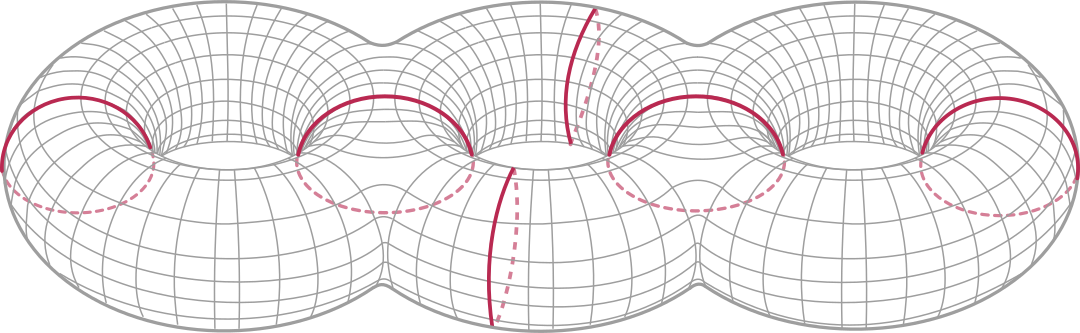
\includegraphics[scale=0.2]{CHARLA_STOCHASTIC_TOPOLOGY_MCG_CIMATNOVEMBER_2018/Pantalones.png}
	\caption{Some essential curves}
\end{figure}

\end{frame}
\begin{frame} \frametitle{The  curve  complex}

And  we  will  put  an edge  connecting  them  if   they  admit  a realization  without  intersection. 

\begin{figure}[h!]
	\centering
	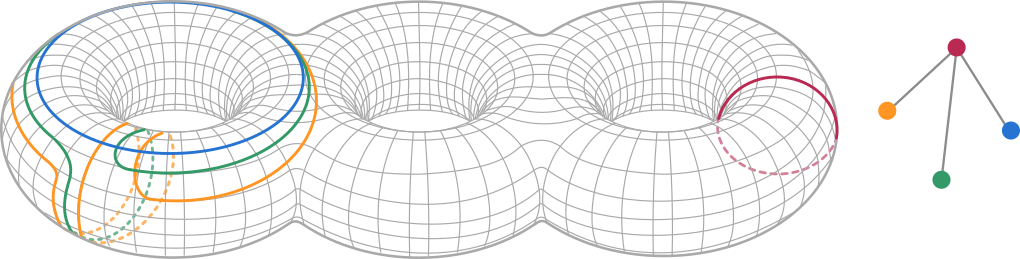
\includegraphics[scale=0.25]{CHARLA_STOCHASTIC_TOPOLOGY_MCG_CIMATNOVEMBER_2018/Locally-infinite.png}
	\caption{Construction of the curve complex}
\end{figure}

One  gets  a simplicial  (flag) complex,  denoted  by $\mathcal{C}(S)$, the  curve  complex. \pause  
\end{frame}
\begin{frame} \frametitle{Rigidity  of  the  Curve  complex}



A homeomorphism $\varphi: S\to  S$,  acts  on the  vertices by  permuting  the isotopy  class  of  the curves. Homeomorphisms which  are  isotopic  to the  identity  act  trivially. 
For  one  second, allow  for   non-orientation-preserving  homeomorphisms as  well. 

\begin{theorem}[Luo]

Let  $S$  be  a  closed  surface  of  genus  at  least  $2$. The (simplicial) automorphisms  of the curve complex $\mathcal{C}$ are  in bijective correspondence  with  isotopy classes of homeomorphisms  of  the  surface.   \pause 
$$Aut(\mathcal{C}(S))\cong Mod^{*}(S).\pause $$
\end{theorem}

\end{frame}

\begin{frame}
\textbf{Here, such classes  are  responsible  for  the  rigidity  phenomenon. The  automorphisms  of  the  curve  complex  are  all geometric.\pause  The  group  of simplicial   automorphism  of  the  curve  complex  is  the  extended  Mapping  Class group. \pause Ivanov's Rigidity  meta-conjecture.}

Version  of  Margulis superrigidity Theorem. 
 

\end{frame}


\begin{frame}

\begin{definition}
The  mapping class group, Mod(S) is the  (discrete!) group  of  (orientation preserving) homeomorphisms of  the  surface, modulo  the subgroup of homeomorphisms  which  are  homotopic  to  the  identity. \pause

$$ Mod(S)= Homeo^{+}(S)\diagup Homeo_{0}(S). \pause $$
(Versions for  a  surface with  a  finite  number  of boundary  components). 
 
 \end{definition}
 \end{frame}
 
\begin{frame}

\begin{example}
\begin{itemize}

\item Let $D^2$ denote  the  2-dimensional  disk. $Mod(D^2)$ is  the  trivial  group. Any orientation preserving  homeo  has  a  fixed  point. \pause It  is homotopic  to  the  identity  via  a  radial homotopy. \pause
\item Let  $A$  be  the  annulus. $Mod(A)$ is  the group  of  integers. \pause 
\item Let $T$ be  the  torus. \pause  $H_1(T)\cong \mathbb{Z}^2$, \pause 
$$Mod(T) \to Aut^{+}(H_{1}(T))\pause = Aut^{+}(\mathbb{Z}^2)\cong Sl_2(\mathbb{Z}) $$ 
\end{itemize}
\end{example}
\end{frame}



\section{Four  properties  of the curve  complex.  }
\begin{frame}
Recall  the  curve  complex, $\mathcal{C}(S)$. Its   vertices  are   isotopy  classes  of  essential  curves. There  is  an  edge  if two  such  curves  have  a  disjoint  realization. 

 \begin{theorem}
Let  $S_g$ be  a  genus  $g$  closed  surface, where  $g$  is t  least $2$. 
The  curve  complex  has  the  following  properties: 
\begin{itemize}
\item  It  is  connected. 
\item Every  vertex  has  infinite degree. 
\item It  has  clique  number  equal  to $3g-3$
\item It  has infinite  diameter.  
\end{itemize}
\end{theorem}
\end{frame}


\section{Main Results}

\begin{frame}\frametitle{Explanation}

Aim  of  this  Effort:  give  Probabilistic  proofs  of properties of  the  curve complex, based  on the  theory  of  random graphs.  \pause 




The  easy  ones: the  four  fundamental  properties  listed above. (Nice  didactical  introduction  to  fundamental   ideas  of  random graph theory). \pause Reason to be delivered here  in the  TDA-Stochastic  topology  School. \pause   
This  gives  probabilistic  proofs  of   results  about  mapping  class  groups.  \pause 

\end{frame}

\begin{frame}

The more  involved  one, but also  adressed here: Luo's proof  of  rigidity  of  the  curve  complex.  \pause 
\end{frame}
\begin{frame}

\textbf{Slogan: The  Curve  complex  is   very  similar  to  a Random Graph  in the  sense  of  Erd\"os-R\'enyi  with  very  specific  parameters,  obtained  in the  limit (The  Rado Graph). \pause }

Deterministic  counterpart: Behring- Gaster's result. 

 




\end{frame}

\begin{frame}\frametitle{Aknowledgements}

\begin{center}
This  is  Ricardo Ch\'avez-C\'aliz  MSc. Thesis, in process at  UNAM. 
\end{center}

Fruitful  insights  from  Octavio Arizmendi, \pause but  also a  group  of  experts on the  curve  complex  and  mapping class  groups (around Jes\'us Hern\'andez) based  in Morelia.

\end{frame}

\begin{frame}
\frametitle{Connectedness}

\begin{theorem}
Let $\omega(n)$ be a function that tends to infinity arbitrarily slow as $n$ tends to infinity
\begin{itemize}
\item If $p\geq \frac{log(n)+ \omega(n)}{n}$ then 
$$\lim_{n \to \infty} \P(G \in \G(n,p) \text{ is connected}) = 1$$
\item If $p\leq \frac{log(n)- \omega(n)}{n}$ then
$$\lim_{n \to \infty} \P(G \in \G(n,p) \text{ is disconnected}) = 1$$
\end{itemize}
\end{theorem}

\end{frame}

\begin{frame}
\frametitle{Vertices have  infinite  degree}
\begin{theorem}
Let $\epsilon>0$ be fixed, $\epsilon n^{-3/2} \leq p = p(n) \leq 1 - \epsilon n^{-3/2}$, let $k = k(n)$ be a natural number and set $\lambda_{k} = \lambda_{k}(n) = n\cdot b(k;n - 1,p)$. Then the following assertions hold.

\begin{itemize}
\item If $\lim \lambda_{k}(n) = 0$, then $\lim P(X_{k} = 0) = 1$. 
\item If $\lim \lambda_{k}(n) = \infty$, then $\lim P(X_{k} > t) = 1$
for every fixed $t$.
\item If $0 < \lim\lambda_{k}(n) < \lim \lambda_{k}(n) < \infty$,
then $X_{k}$ has asymptotically Poisson distribution with mean $\lambda_{k}$: 
$$P(X_{k} = r) \sim e^{\lambda_{k}}\cdot \lambda_{k}^{r}/ r!$$
for every fixed $r$.
\end{itemize}
\end{theorem}
\end{frame}

\begin{frame}

\frametitle{Clique Number  and asymptotic  of  genera.}
\begin{theorem}
Let $r = r(n) = O(n^{1/3})$ and let $p=p(n)$, $0<p<1$, be such that
$$\binom{n}{r} p^{\binom{r}{2}} \to \infty \text{ and } \binom{n}{r+1} p^{\binom{r+1}{2}} \to 0 $$
Then a.e $G_{p}$ has clique number $r$
\end{theorem}
\end{frame}

\begin{frame}\frametitle{Infinite  diameter}
\begin{theorem}
Let $c$ be a positive constant, $d=d(n)\geq 2$ a natural number, and define $p=p(n,c,d), 0<p<1$, by
$$p = \frac{\big( n\cdot log(n^2/c)\big) ^{1/d}}{n}$$
Suppose that $pn/(log\text{ }n)^{3} \to \infty$. Then in $G(n,p)$ we have
$$\lim_{n\to \infty} \P (diam\text{ }G = d) = e^{-c/2} \text{ and }  \lim_{n\to \infty} \P (diam\text{ }G = d+1) = 1 - e^{-c/2}$$
\end{theorem}
\end{frame}


\section{Rigidity }
\begin{frame}

\end{frame}

\end{document}

